\chapter{The Standard Model}
\begin{section}{Overview and Successes}

The Standard Model (SM) of particle physics is a wildly successfull theory and one of the greatest accomplishments in science.
Formulated in the second half of the 20th century, it describes 17 experimentally-observed, fundamental particles and their interactions through the electromagnetic, weak, and strong fundamental forces.
These particles, shown in Figure~\ref{fig:sm_particles}, consist of six quarks and six leptons, known as fermions, which comprise the matter particles, along with four gauge bosons and one scalar boson, which mediate particle interactions.

\begin{figure}[tbp!]
\begin{center}
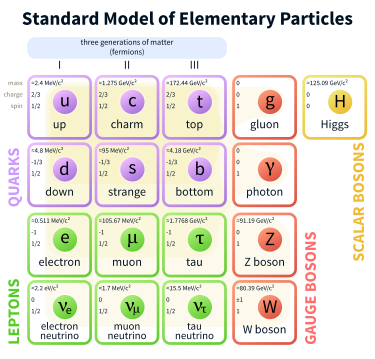
\includegraphics[angle=0,width=0.80\columnwidth]{fig/sm_particles.png}
\end{center}
\caption{The fundamental particles of the Standard Model and some of their properties.}
\label{fig:sm_particles}
\end{figure}

Formally, the Standard Model is quantum field theory with symmetries described by the group $\mrm{SU}_c(3) \times \mrm{SU}_L(2) \times \mrm{U}_Y(1)$ and with a Lagrangian of
\begin{align}
\mathcal{L} &= -\frac{1}{4}F_{\mu\nu}F^{\mu\nu} \nonumber + i\overline{\psi}_i\slashed{D}\psi_i \\
            &+ \psi_{i}y_{ij}\psi_{j}\phi + h.c. \nonumber + |D_{\mu}\phi|^2 - V(\phi),
\end{align}
where $F_{\mu\nu}$ is the field strength tensor, $D_{\mu}$ is the gauge covariant derivative, $\slashed{D} = \gamma^{\mu}D_{\mu}$, $\psi_{i}$ are the fermion fields, $\phi$ is the Higgs field, $y_{ij}$ are the yukawa couplings, and h.c. is the hermitian conjugate of the term directly preceeding it.
In the top line, the first term of the Lagrangian describes the interactions of gauge bosons, while the second encodes the interactions between gauge bosons and fermions.
The bottom line describes Higgs physics with the first term describing the Higgs-fermion interactions, the second term encoding the Higgs-gauge boson interactions, and finally, the third term representing the Higgs potential.

As the Standard Model is able to provide predictions across an enormous scope of physics, it has been rigorously tested throughout its history.
For example, Figure~\ref{fig:sm_tests}, shows the agreement between the SM predictions and experimental results for the production cross section of a variety of processes.
Amazingly, all of the measurements, spanning nine order sof magnitude, agree with SM predictions.
At the same time, the Standard Model is the most precisely tested theory in physics with its prediction~\cite{PhysRevLett.109.111807} of the anamalous electron magnetic moment incredibly agreeing with experimental measurements~\cite{PhysRevLett.100.120801,PhysRevA.83.052122} at up to fourteen decimal places, as shown in Table~\ref{tab:ae_values}.

\begin{figure}[tbp!]
\begin{center}
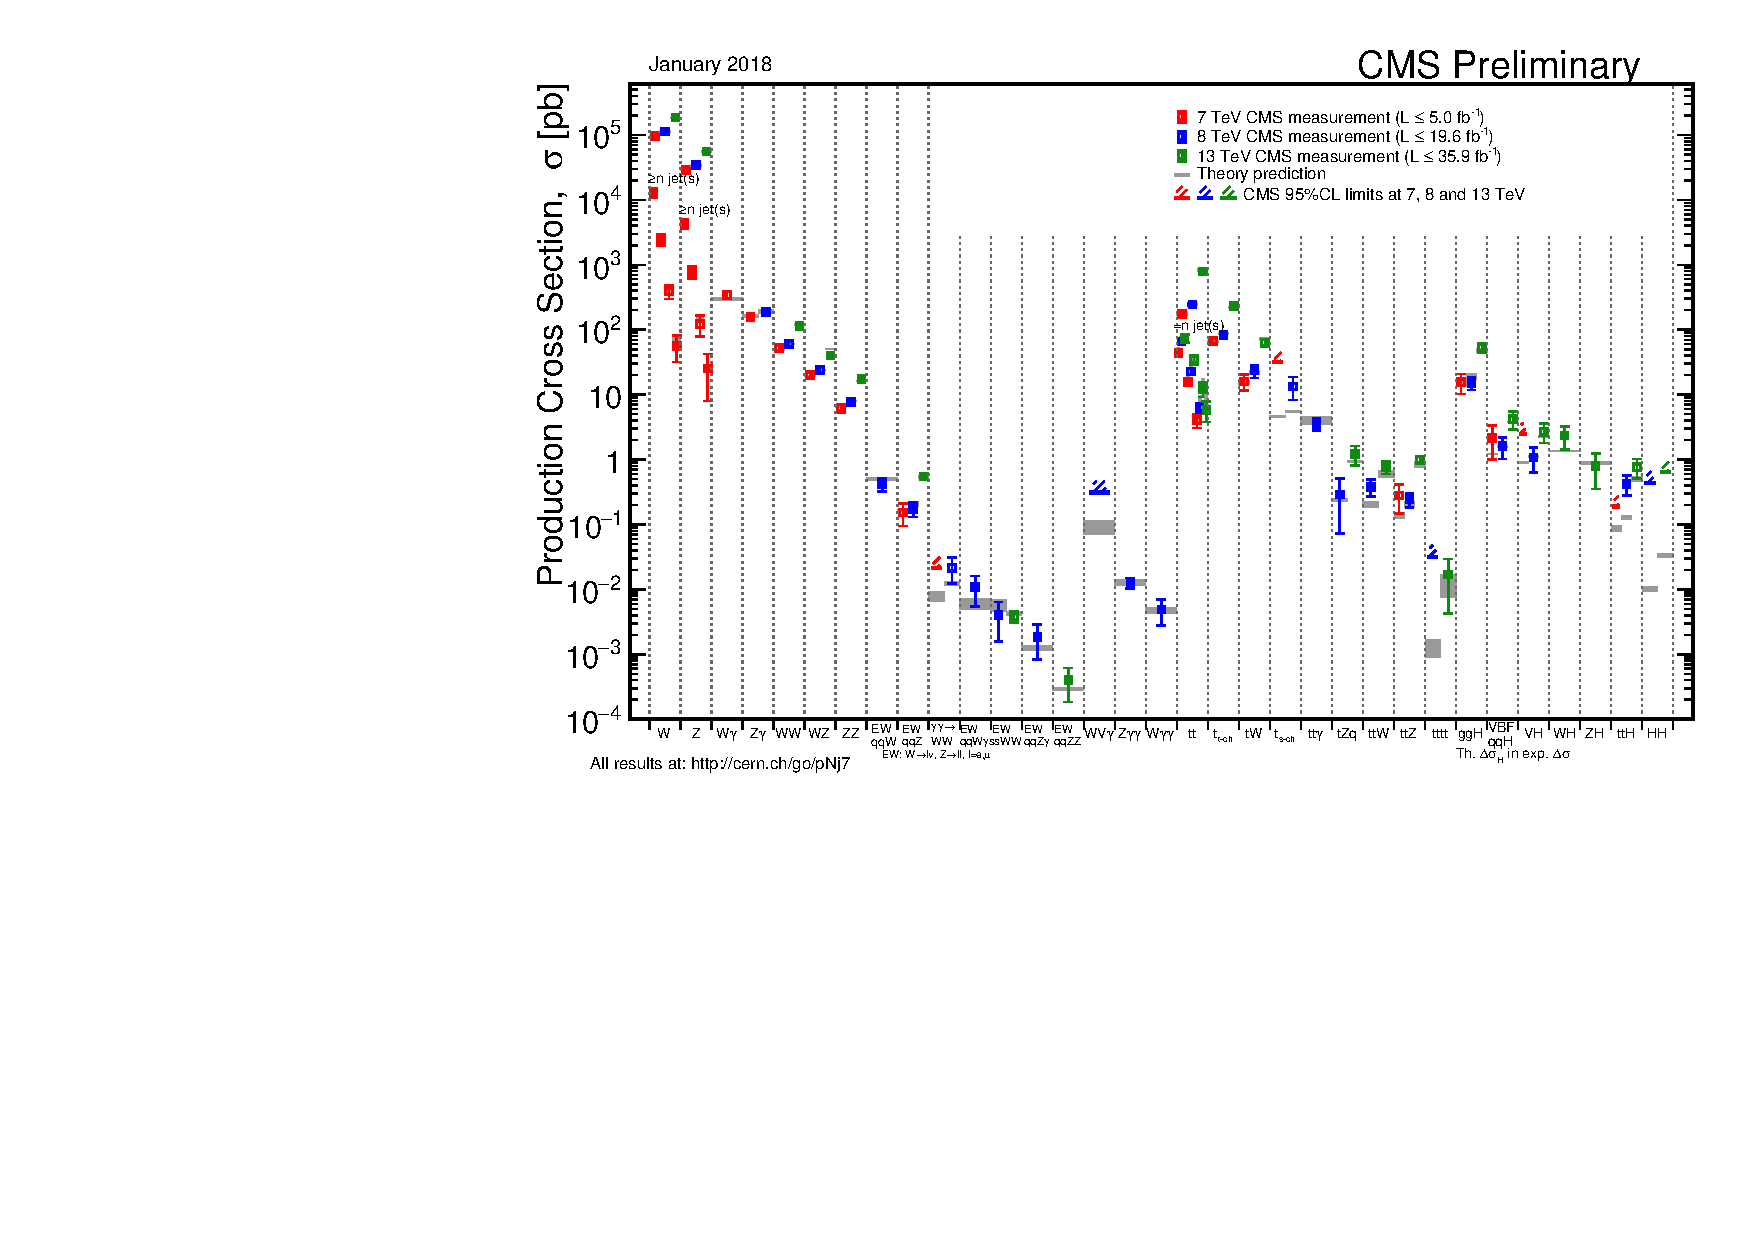
\includegraphics[angle=0,width=0.95\columnwidth]{fig/sm_tests.pdf}
\end{center}
\caption{The theoretical and experimental value for the production cross section of various processes~\cite{sm_tests}.}
\label{fig:sm_tests}
\end{figure}

\begin{table}[tbp!]
\centering
\begin{tabular}{ |c|c| }
\hline
$a_e \mrm{(Theory)}$      &  0.001 159 652 181 78(77) \\
$a_e \mrm{(Experiment)}$  &  0.001 159 652 180 73(28) \\
\hline
\end{tabular}
\caption{The theoretical~\cite{PhysRevLett.109.111807} and experimental~\cite{PhysRevLett.100.120801,PhysRevA.83.052122} values of the anamalous electron magnetic moment, $a_e$.
The uncertainty in the last digits is shown in parantheses.}
\label{tab:ae_values}
\end{table}

\end{section}

\begin{section}{The Standard Model as an Incomplete Theory}

Despite the impressive successes of the Standard Model, it is incomplete as a fundamental description of the unvierse and many tensions exist between it and both experimental and theoretical concerns.
For example, the Standard Model glaringly leaves out the fundamanetal force of gravity and attempts to construct a theory of quantum gravity have been frought with difficulties.
Furthermore, the Standard Model is unable to explain the substantial astrophysical evidence for dark matter~\cite{Bertone:2004pz,Rubin:1970zza}, which comprises $\sim 80\%$ of the matter in the universe, as it has no suitable candidate that can account for the observed mass density of dark matter.

Additionally, the Standard Model provides no mechanisms for:
\begin{itemize}
\item the origin of neutrino masses
\item the matter-antimatter symmetry
\item the presence of dark energy
\item a grand unified theory of the strong and electroweak forces
\end{itemize}

Because of these issues, the Standard Model is believed to be a low-energy effective field theory with new physics entering at higher energies.
It is, however, not easy to know what form this new physics may take, and thus solutions to the above problems have been used to drive much of the theoretical framework for extending the Standard Model.
In particular, the Hierarchy Problem and the idea of ``naturalness'', described in the section below, are, perhaps, the most significant lampposts in the search for new physics.

\begin{subsection}{The Hierarchy Problem and Naturalness}

The long-awaited discovery of the Higgs boson~\cite{Aad:2012tfa,Chatrchyan:2012xdj,Chatrchyan:2013lba,Khachatryan:2014jba,Aad:2014aba,Aad:2015zhl} confirmed the existence of a scalar boson with an observed mass of approximately $125~\GeV$.
This relatively low mass of the Higgs boson, however, creates two related theoretical concerns.
First, the Higgs mass is tied to the electroweak scale by the relation 
\begin{align}
v = \frac{\mh}{\sqrt{2}\lambda_h} \approx 246~\GeV
\end{align}
where $v$ is the higgs vacuum expectation value (vev), $m_H$ is the physical Higgs mass, and $\lambda_h$ is the Higgs Yukawa coupling.
The vev directly dictates the electroweak scale and is only on the order of 100~\GeV.
The next largest known energy scale is that of quantum gravity and is typically defined as the Planck mass, which is on the order of $10^{19}~\GeV$.
The question as to why these two scales are so discrepant is known as the Hierarchy Problem~\cite{Barbieri:1987fn}.

The second question stems from trying to understand the observed mass of the Higgs boson in the prescence of quantum corrections.
The Higgs mass can be broken down into two components, its bare mass, $m_{H,0}$, and contributions from radiative corrections, $\delta m_H^2$, as shown in the equation below
\begin{align}
\mh^2 = m_{H,0}^2 + \delta \mh^2.
\end{align}
As a scalar particle, the Higgs boson mass receives contributions from all massive particles, and in partcular, for a fermion, $f$, the contribution to the Higgs mass at the one-loop level, corresponding to the the diagram shown in Figure~\ref{fig:higgs_fermion_loop}, is of the form
\begin{align}
\delta \mh^2|_f &= -\frac{\lambda^2_f}{8\pi^2}N_f \int^{\Lambda_{UV}} \frac{d^4p}{p^2} \nonumber \\
                &= -N_f\frac{\lambda^2_f}{8\pi^2 } \left[\Lambda^2_{UV} - 6m_f^2\ln\left(\frac{\Lambda_{UV}}{m_f}\right) + 2m_f^2\right] + \mathcal{O}\left(\frac{1}{\Lambda^2}\right),
\label{eqn:higgs_fermion_correction}
\end{align}
with $\lambda_f$ the Yukawa coupling and $N_f$ the number of fermionic degrees of freedom.
The quantity $\Lambda_{UV}$ is the cutoff of the momentum integral, which represents the approximate scale at which the Standard Model is no longer valid.
In the case that there is no new physics beyond the Standard Model, this would correspond to $\Lambda_{UV} \sim \text{Planck scale} \sim 10^{19}~\GeV$, where effects due to quantum gravity are introduced.

\begin{figure}[tbp!]
\begin{center}
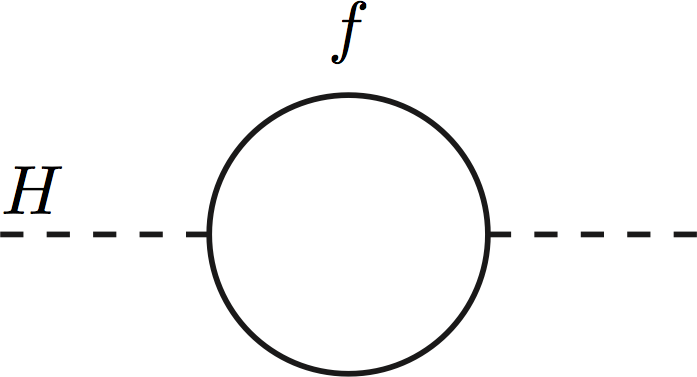
\includegraphics[angle=0,width=0.40\columnwidth]{fig/higgs_fermion_loop.png}
\end{center}
\caption{The fermionic one-loop Higgs mass correction.}
\label{fig:higgs_fermion_loop}
\end{figure}

In this scenario, the leading term of the Higgs mass corrections is $\mathcal{O}(10^{38}~\GeV^2)$, while, as measured, the squared Higgs mass is only $\mathcal{O}(10^{4}~\GeV^2)$.
For these two values to be consistent with each other, the Higgs bare mass parameter must exactly cancel the correction term at over 30 decimal places of precision.
This high-level of fine-tuning is considered to be ``unnatural'' and has been deemed the Naturalness Problem~\cite{Feng:2013pwa,Craig:2013cxa,Papucci:2011wy,Casas:2014eca}.
While it is entirely plausible that such a fine-tuned cancellation of parameters occurs -- there is no inherent theoretical reason against this, this problem motivates the need for new physics below the Planck scale, particularly physics that naturally incorporates a mechanism for cancelling the quadratic divergence of the $\Lambda_{UV}^2$ term.

\end{subsection}

\end{section}
